% !TeX root = Protokoll.tex
\subsection{Vermessung der Moden}
Die zur Untersuchung der drei Moden aufgenommenen Reflektorspannungen für die rechten und linken Nullstellen 
sowie das Maximum der Amplitude sind in \cref{tab:Moden} eingetragen. Die Frequenz der jeweiligen Mode 
ist ebenfalls angegeben.
\FloatBarrier
\begin{table}[!h]
	\centering
	\begin{tabular}{ccccc}
		\toprule
		Reflektorspannung & Reflektorspannung & Reflektorspannung & Amplitude & Frequenz\\
		$U_0$/\si{V} & $U_1$/\si{V} & $U_2$/\si{V} & $A$/\si{Teilstrich} & $f_0$/\si{MHz}\\
\midrule
		\num{155} & \num{140} & \num{170} & \num{5.800} & \num{9143}\\
		\num{235} & \num{220} & \num{245} & \num{5.300} & \num{9142}\\
		\num{100} & \num{90} & \num{110} & \num{4.600} & \num{9148}\\
		\bottomrule
	\end{tabular}
	\caption{Messwerte für die Reflektorspannungen, bei denen das Maximum ($U_0$),
                 der linke Einstiegswert ($U_1$) und der rechte Einstiegswert ($U_2$)
                 am festgelegten Referenzpunkt auf dem Oszilloskop lagen.
                 Für alle drei Moden sind die jeweilige Amplitude und Frequenz angegeben.
                 \label{tab:Moden}}
\end{table}

\FloatBarrier
Die grafische Darstellung dieser Messwerte ist in \cref{fig:modenkurven} zusammen mit den angedeuteten 
Modenkurven gegeben.
\FloatBarrier
\begin{figure}[!h]
 \centering
 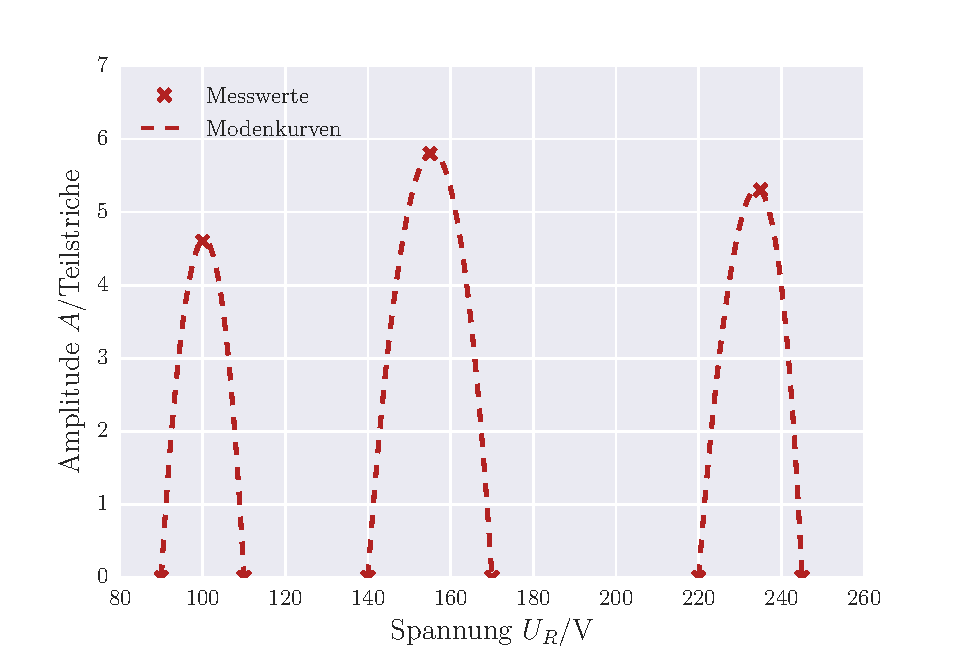
\includegraphics[scale=0.9]{../Grafiken/Modenkurven.pdf}
 \caption{Grafische Darstellung der aufgenommenen Messwerte für die Amplituden der Modenkurven in 
 	Abhängigkeit der eingestellten Reflektorspannung. Aufgrund der geringen Messpunktanzahl sind Verläufe der 
 jeweiligen Modenkurven nur angedeutet. \label{fig:modenkurven}}
 \end{figure} 
\FloatBarrier
Die aufgenommenen Frequenzen und Reflektorspannungen bei denen die zu beobachtende Einsattelung im Maximum 
und dem linken und rechten Halbwert des Maximums lag, sind in \cref{tab:Elektrische Abstimmung} angegeben.
\FloatBarrier
\begin{table}[!h]
	\centering
	\begin{tabular}{cc}
		\toprule
		Reflektorspannung & Frequenz\\
		$U_0$/\si{V} & $f_0$/\si{MHz}\\
\midrule
		\num{60} & \num{9152}\\
		\num{50} & \num{9120}\\
		\num{65} & \num{9192}\\
		\bottomrule
	\end{tabular}
	\caption{Messwerte der Reflektorspannung, mit Einsattelung im Maximum
                    und in der linken und rechten Halbwert des Maximums mit den 
                    entsprechend eingestellten Frequenzen.
                 \label{tab:Elektrische Abstimmung}}
\end{table}

\FloatBarrier
Aus diesen lässt sich die elektrische Bandbreite $\Delta f_{\mathrm{E}}$, nach \eqref{eq:Bandbreite}, zu 
\begin{empheq}{equation}
	\Delta f_{\mathrm{E}} = \SI{72(1)}{MHz}
\end{empheq}
bestimmen. Aus dieser ergibt sich der Wert der Abstimmempfindlichkeit $E$ mit \eqref{eq:Abstimmempfindlichkeit} zu
\begin{empheq}{equation}
E = \SI{5(2)}{\MHz\per\volt}.
\end{empheq}
\subsection{Bestimmung der Frequenz und Dämpfung}\label{sec:Frequenz_Daempfung}
Die beiden Positionen der Minima und die am Frequenzmesser eingestellte Frequenz sind in \cref{tab:Frequenzmessung}
angegeben.
\FloatBarrier
\begin{table}[!h]
	\centering
	\begin{tabular}{ccc}
		\toprule
		Frequenz & Pos. 1.Minimum & Pos. 2.Minimum\\
		$f_0$/\si{MHz} & $d_1$/\si{mm} & $d_2$/\si{mm}\\
\midrule
		\num{9144(1)} & \num{72.0(1)} & \num{96.0(1)}\\
		\bottomrule
	\end{tabular}
	\caption{Messwerte der Positionen von zwei aufeinander folgenden Minima, 
	mit entsprechender Frequenz. 
                 \label{tab:Frequenzmessung}}
\end{table}

\FloatBarrier
Der doppelte Abstand der Minima entspricht der Wellenlänge im Hohlleiter $\lambda_g$. Diese ergibt sich 
mit den Messdaten zu 
\begin{empheq}{equation}
	\lambda_g = \SI{48.0(3)}{mm}.
\end{empheq}
Mit Hilfe von \eqref{eq:Hohlleiter_Frequenz} und der gemessenen Breite des Hohlleiters $a = \SI{22.70(5)}{mm}$
erhält man die Frequenz im Hohlleiter zu 
\begin{empheq}{equation}
f = \SI{909(3)e7}{Hz}.
\end{empheq}

Die aufgenommenen Messwerte für die Dämpfung am SWR-Meter und die Einstellung des Mikrometers sind
in \cref{tab:Daempfung} zusammen mit den entsprechenden Dämpfungen aus der Eichkurve des Dämpfungsglieds eingetragen.
\FloatBarrier
\begin{table}[!h]
	\centering
	\begin{tabular}{ccc}
		\toprule
		SWR-Meter Ausschlag & Mikrometer & Dämpfung Eichkurve\\
		$\mathrm{SWR}$/\si{dB} & $d$/\si{mm} & $D$/\si{dB}\\
\midrule
		\num{0} & \num{0.43(1)} & \num{1(1)}\\
		\num{2} & \num{1.97(1)} & \num{8(1)}\\
		\num{4} & \num{2.23(1)} & \num{10(1)}\\
		\num{6} & \num{2.55(1)} & \num{12(1)}\\
		\num{8} & \num{2.72(1)} & \num{14(1)}\\
		\num{10} & \num{2.92(1)} & \num{16(1)}\\
		\bottomrule
	\end{tabular}
	\caption{Aufgenommene Dämpfungswerte vom SWR-Meter und die jeweilige Einstellung
                des Mikrometers am Dämpfungsglied, mit der entsprechenden Dämpfung aus der Eichkurve.
                Für die Werte des SWR-Meters sind keine Fehler angegeben, da zwischen Werte auf der verwendeten
                Skala nur schwierig abzulesen waren. \label{tab:Daempfung}}
\end{table}

\FloatBarrier
Die Messwerte der Dämpfung am SWR-Meters sowie die der Eichkurve sind in \cref{fig:daempfung} grafisch dargestellt.  
\FloatBarrier
\begin{figure}[!h]
 \centering
 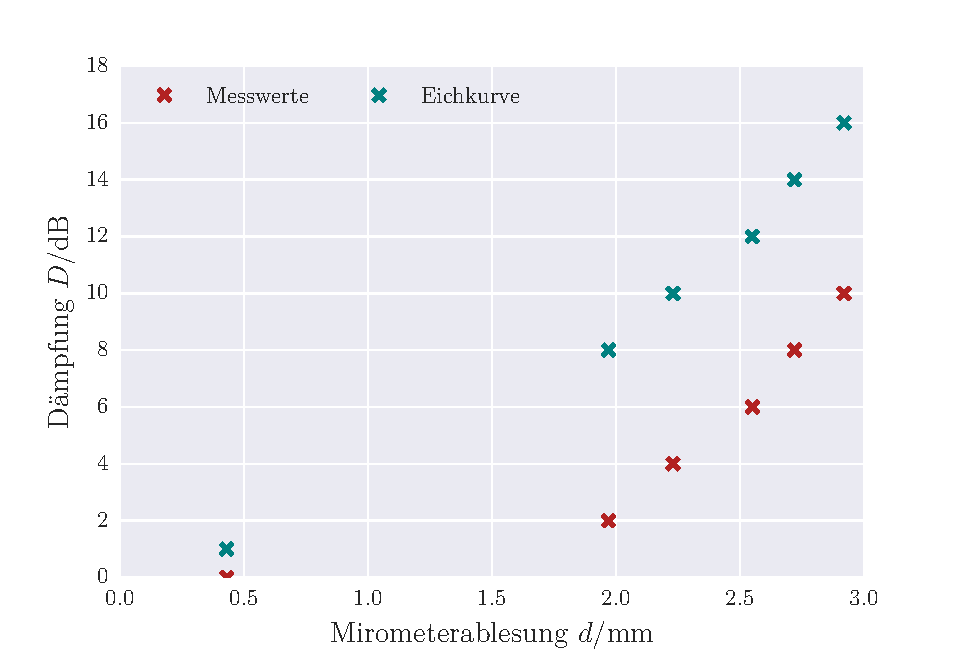
\includegraphics[scale=0.9]{../Grafiken/Daempfung.pdf}
 \caption{Darstellung der Abhängigkeit der Dämpfung am SWR-Meter von der Mikrometereinstellung am Dämpfungsglied im Vergleich
 	zu der jeweilig eingestellten Dämpfung aus der Eichkurve am Dämpfungsglied.
 	  \label{fig:daempfung}}
 \end{figure} 
\FloatBarrier
\subsection{Bestimmung des Stehwellenverhältnisses}
In \cref{tab:SWR_Meter} sind die mit dem SWR-Meter gemessenen Werte des Stehwellenverhältnisses in Abhängigkeit der
Sondentiefe am Gleitschraubentransformator angegeben. 
\FloatBarrier
\begin{table}[!h]
	\centering
	\begin{tabular}{cc}
		\toprule
		Sondentiefe & SWR-Meter Ausschlag\\
		$s$/\si{mm} & $\mathrm{SWR}$\\
\midrule
		\num{3.00(1)} & \num{1.12}\\
		\num{5.00(1)} & \num{1.30}\\
		\num{7.00(1)} & \num{3.00}\\
		\num{9.00(1)} & \num{9.00}\\
		\bottomrule
	\end{tabular}
	\caption{Messwerte des vom SWR-Meter gemessenen Stehwellenverhältnisses in Abhängigkeit der Sondentiefe 
                am Gleitschraubentransformator. \label{tab:SWR_Meter}}
\end{table}

\FloatBarrier
Die 3dB-Punkte um ein Minimum der Mikrowelle, die zur Bestimmung des Stehwellenverhältnisses gemessen wurden sind 
in \cref{tab:SWR_3dB_Methode} zusammen mit den Positionen zweier aufeinander folgender Minima angegeben. 
\FloatBarrier
\begin{table}[!h]
	\centering
	\begin{tabular}{cccc}
		\toprule
		3dB-Punkt & 3dB-Punkt & Pos. 1.Minimum & Pos. 2.Minimum\\
		$d_1$/\si{mm} & $d_2$/\si{mm} & $d_1$/\si{mm} & $d_2$/\si{mm}\\
\midrule
		\num{88.600} & \num{87.700} & \num{96} & \num{76}\\
		\bottomrule
	\end{tabular}
	\caption{ Messwerte der Positionen des linken (1) und rechten (2) 3dB Punktes um ein Minimum
                    und derer zweier auf einander folgender Minima. \label{tab:SWR_3dB_Methode}}
\end{table}

\FloatBarrier
Aus den Positionen der Minima lässt sich wie in \cref{sec:Frequenz_Daempfung} die Wellenlänge im Hohlleiter
als der doppelte Abstand der beiden Minima bestimmen.
Diese ergibt sich zu:
\begin{empheq}{equation}
\lambda_g = \SI{40.0(3)}{mm}	
\end{empheq} 
Mit dieser und den 3dB-Punkten kann nun das Stehwellenverhältnis nach \eqref{eq:SWR_3dB} bestimmt werden.
Man erhält den genäherten Wert des Stehwellenverhältnisses zu:
\begin{empheq}{equation}
S = \num{11.5(2)}
\end{empheq} 

Bei der Messung des Stehwellenverhältnisses mit der Abschwächer-Methode wurden die Dämpfungseinstellungen
$A1 = \SI{20}{dB}$ und $A2 = \SI{5}{dB}$ gemessen. Aus Gleichung \eqref{eq:SWR_Abschwaecher} berechnet sich 
das Stehwellenverhältnis $S$ zu:
\begin{empheq}{equation}
	S = \num{ 7.5(7)}	
\end{empheq} 